\chapter{Results}

This chapter will present the partial results we obtained in this project. First, we will present the different technologies we used in producing droplets and how we overcame arising technical challenges. Then we introduce how we identified an antibiotic producer and its respective target using halo assays to conduct a library screening. Lastly we focus on biological problems which arose due to the unique nature of the droplet environment and issues with the chosen antibiotic production strain in general which led us to conclude the project. 

\section{Successful droplet production}
\begin{figure}
\centering
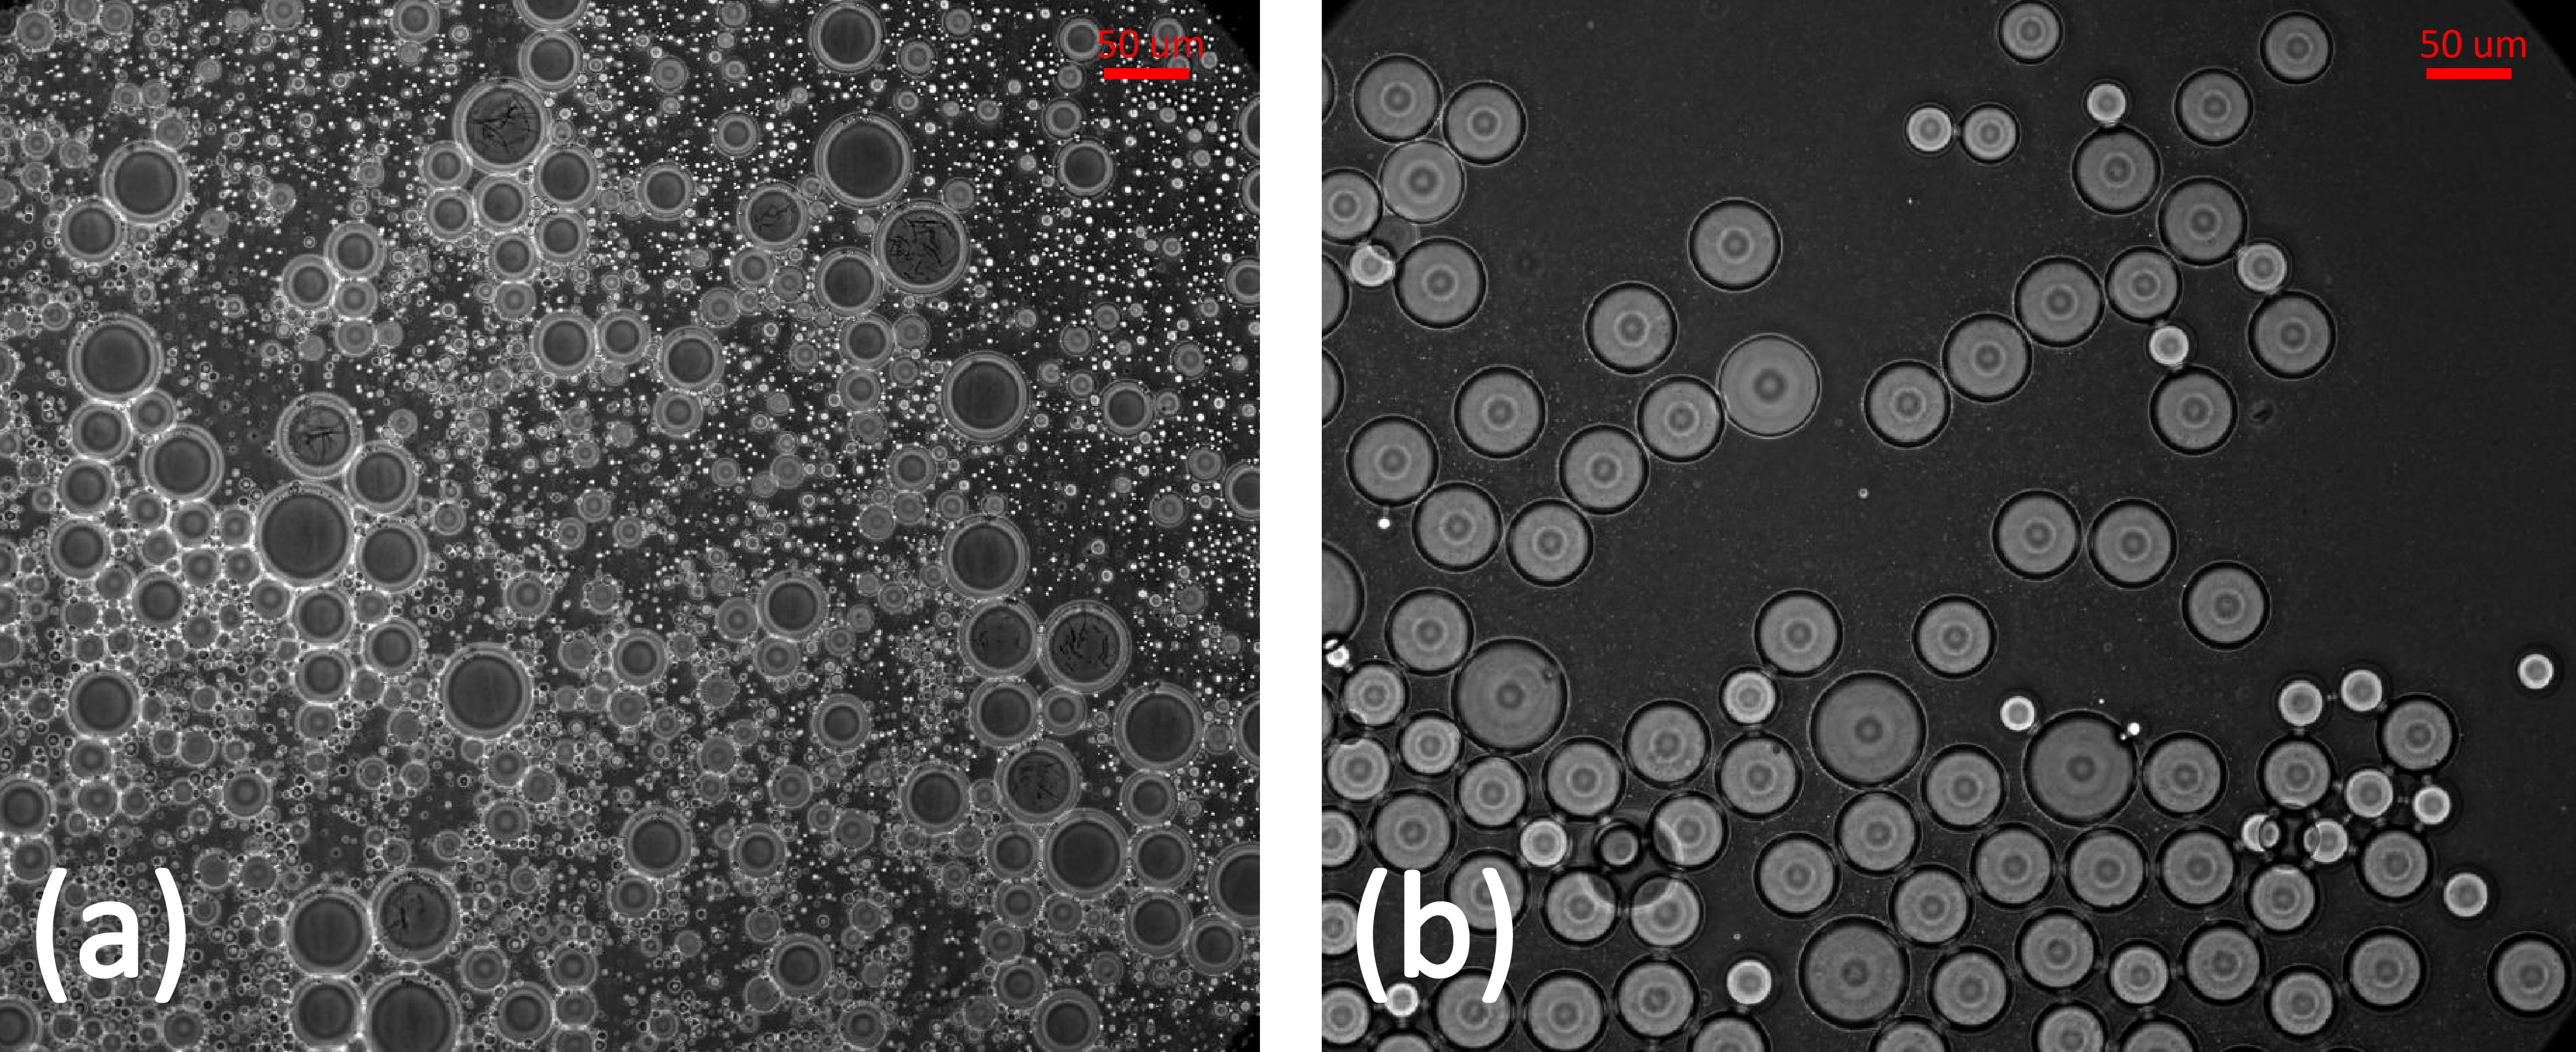
\includegraphics[width=\linewidth]{graphics/2025_09_30_droplets_fig5.png}
\caption{\textbf{Comparison of bulk droplets and on-chip droplets reveals broad size distribution in bulk droplets and narrow size distribution in on-chip droplets} In (a) we see bulk microdroplets after 21h of incubation (30$^\circ$C). A broad distribution of droplet sizes can be observed. In bigger droplets, bacteria are observed. In (b), we see on-chip microdroplets. These are more uniform in size, especially a lower size limit can be observed and the bigger droplets are probably merged single droplets.}
\label{fig:results_droplet_bulk_vs_chip}
\end{figure}
We employed both methods, described in sections~\ref{sec:method_bulk_droplets}~and~\ref{sec:method_chip_droplets}, to produce droplets successfully.~Figure~\ref{fig:results_droplet_bulk_vs_chip} shows the resulting droplets from employing both methods. When using magnetic stirrers to create bulk droplets, we obtain stable microdroplets which are stable even over longer periods of time and incubation. The size distribution is very broad and the upper limit allows significant bacterial growth in droplets~(Figure~\ref{fig:results_droplet_bulk_vs_chip}a). In contrast to this method, when using a commercially available microfluidic chip, we can produce droplets with a very narrow size distribution~(Figure~\ref{fig:results_droplet_bulk_vs_chip}b). These droplets also allow for bacterial growth but producing the droplets is more challenging due to sensitivity of pressures and possible accumulation of debris in the chip which can block production. Nevertheless, for our pilot experiments we use the microfluidic chip to improve reproducibility of droplets and experiments.

\section{Recommended oil evaporates rapidly}
\begin{figure}
\centering
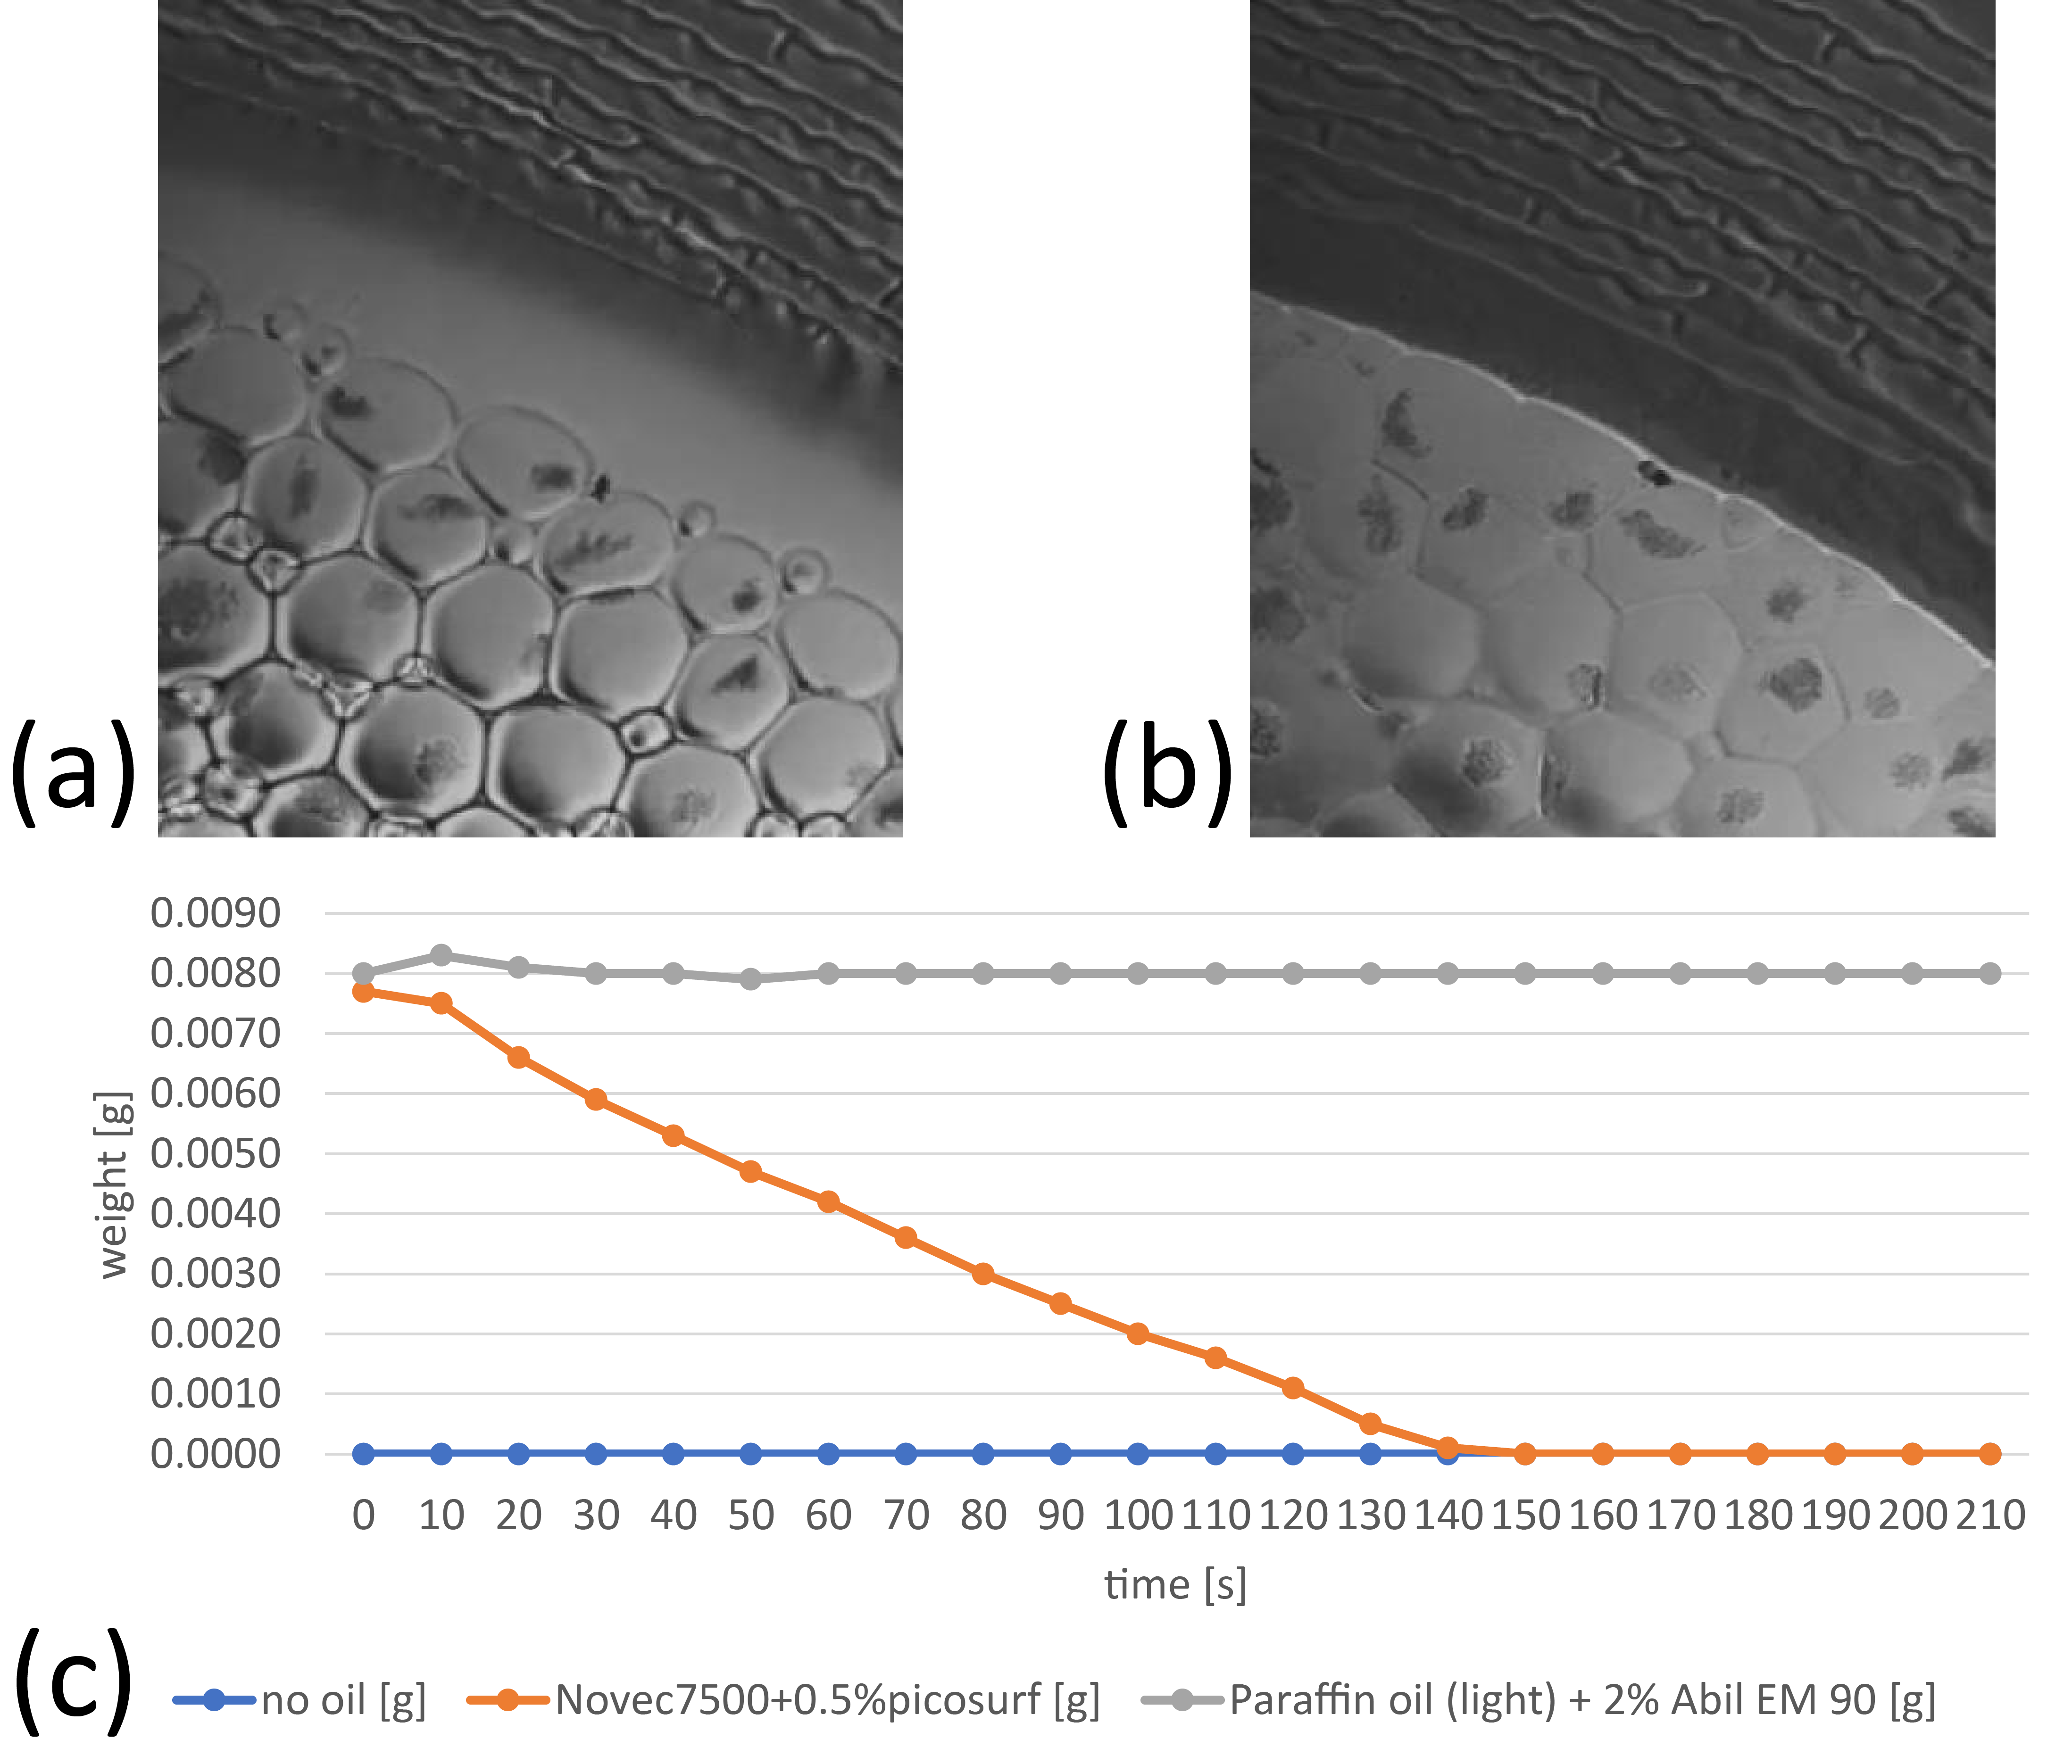
\includegraphics[width=\linewidth]{graphics/2025_09_30_droplets_fig6.png}
\caption{\textbf{Novec\textsuperscript{TM}7500 rapidly evaporates and does not allow for droplet incubation and observation} Using a recommended oil for the commercial microfluidic chip we used, we observed oil evaporation. (a) and (b) show two snapshots of droplets after 21h of incubation in a sealed flask upon placing under the miroscope. The oil recedes (a) until it completely evaporates and the droplets merged (b). Measuring the oil weight on a scale shows a decrease of oil over time (c) while Paraffin oil does not evaporate on the same time scale.}
\label{fig:results_oil_evaporation}
\end{figure}
While we were able to produce stable, observable droplets using Paraffin oil, we did not succeed to observe droplets using Novec\textsuperscript{TM}7500 which was recommended by the manufacturer of our microfluidic chip. Interestingly, we were able to produce droplets and incubate them over long time. Yet, upon exposure to air, the oil exhibited wave dynamics when observed under a microscope (Figure~\ref{fig:results_oil_evaporation}a) and after a short time, the droplets got pushed together and finally surface tension led to collapse and merging of the distinct droplet environments (Figure~\ref{fig:results_oil_evaporation}b). This led us to suspect that the oil might evaporate in our conditions and indeed, when using a glass slide on a high-precision scale and adding a $5 \mu l$ drop of oil, we observe a rapid weight loss, indicating evaporation. For Paraffin oil, which we also use to create droplets, we do not observe this phenomenon~(Figure~\ref{fig:results_oil_evaporation}c). Thus, we focused on producing droplets solely with Paraffin oil.

\section{Identifying producer-target pair}
\begin{figure}
\centering
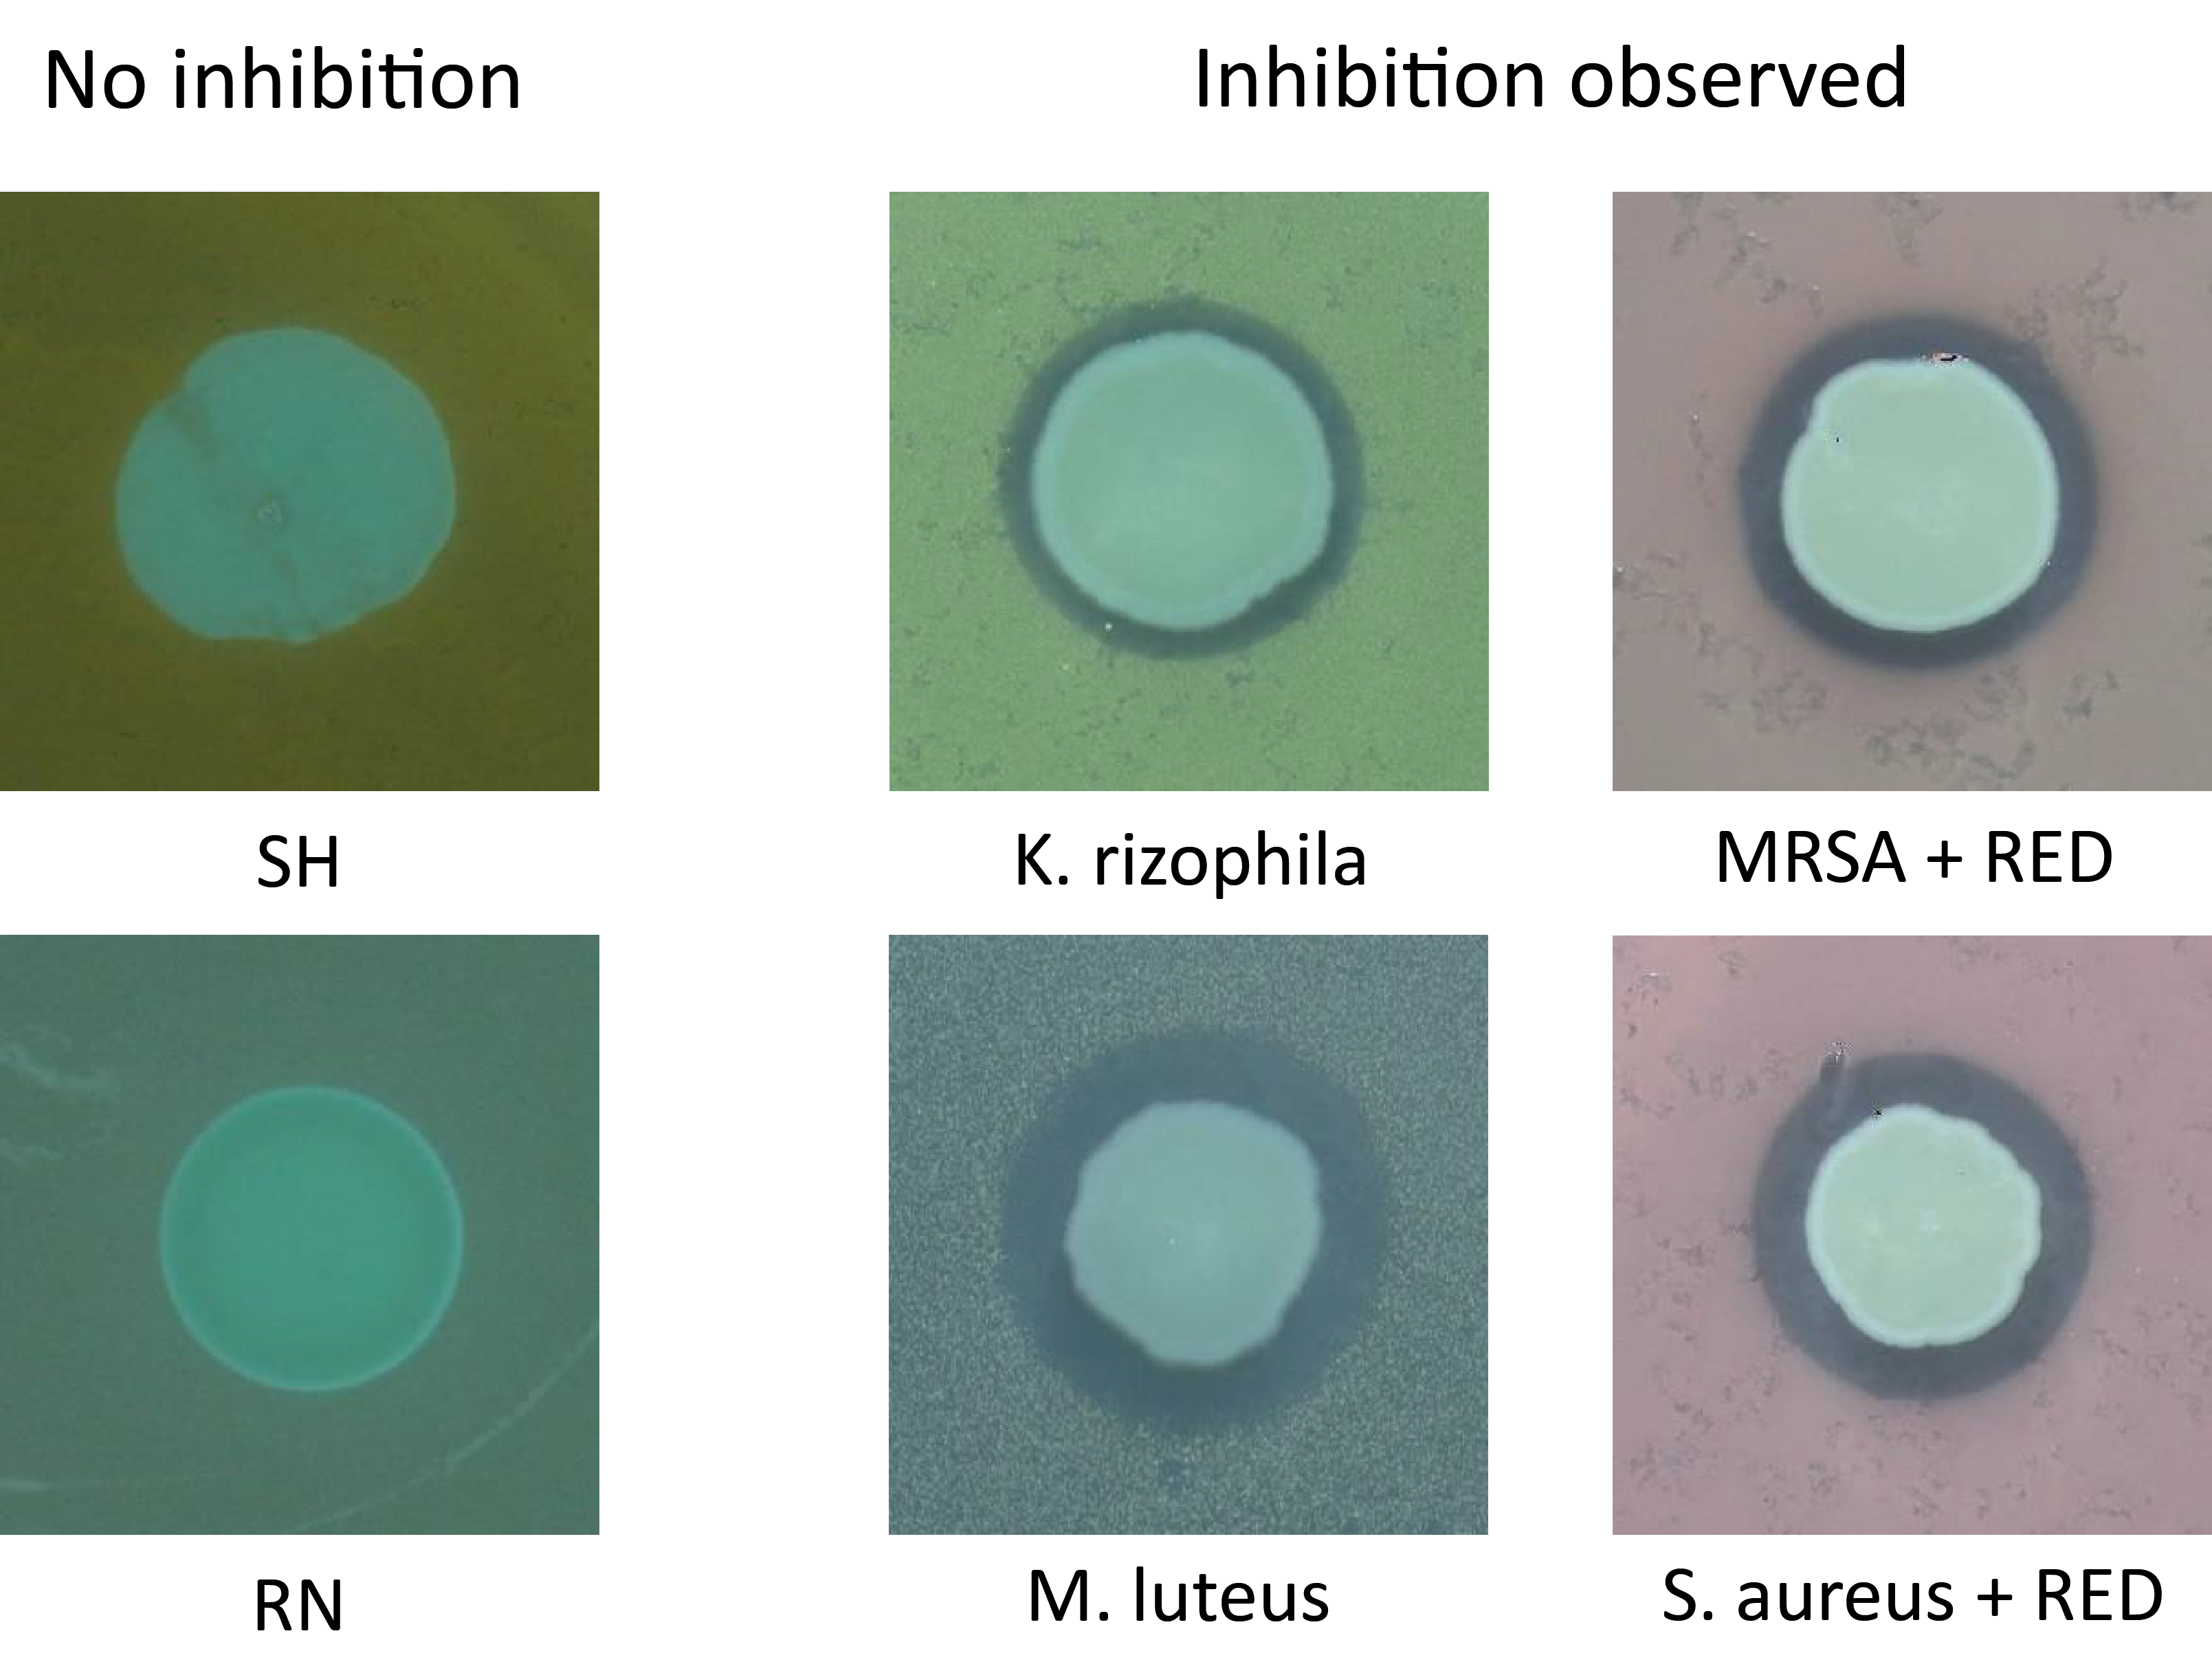
\includegraphics[width=\linewidth]{graphics/2025_09_30_droplets_fig7.png}
\caption{\textbf{Halo assay for library of target strains identifies \textit{Staphylococcus aureus} as potential target} Using halo assays, we conducted a broad screening of very distinct bacterial strains to determine possible target strains for the chosen \textit{Bacillus subtilis} producer strain. Some natural isolates from our collection showed no inhibition but we observed several strains which exhibit inhibition. Among them the commonly used susceptibility test strain of \textit{Kocuria rhizophila} but also clinically relevant strains of \textit{S. aureus}, both methicillin-resistant (MRSA) and sensitive.}
\label{fig:results_sensitive_screening}
\end{figure}
Previous research in our lab~\cite{Gerardin2016-ac} used a colicin-producing \textit{E. coli} strain as an antibiotic producing strain. This is less feasible in droplets due to the inherent nature of colicin. In order for bacteria to release colicin, these bacteria need to lyse~\cite{Cascales2007-oj}. As the volume in droplets is very limited, we inoculate the droplets with low numbers of bacteria. The need of lysis does not allow to use colicin in our setup.
Instead we focused on other antibiotics, based on several criteria like culturability in growth media also suitable for possible target strains, small molecule antibiotics, to allow for beneficial mutations and some hydrophilicity to avoid diffusion outside of the droplets. Based on these criteria, we chose a subtilin-producing \textit{B. subtilis} strain~\cite{Stein2002-nv, Zhang2022-ee} as the antibiotic producing strain.
After choosing our antibiotic producing strain, we screened a collection of possible target strains, selected based on similar growth rate and easy culture conditions using halo assays. We observe inhibition for several of the possible targets~(Figure~\ref{fig:results_sensitive_screening}). Based on these results, we chose a \textit{Staphylococcus aureus} strain due to the large inhibition zone combined with its clinical significance.

\section{\textit{Bacillus subtilis} stressed in droplets}
\begin{figure}
\centering
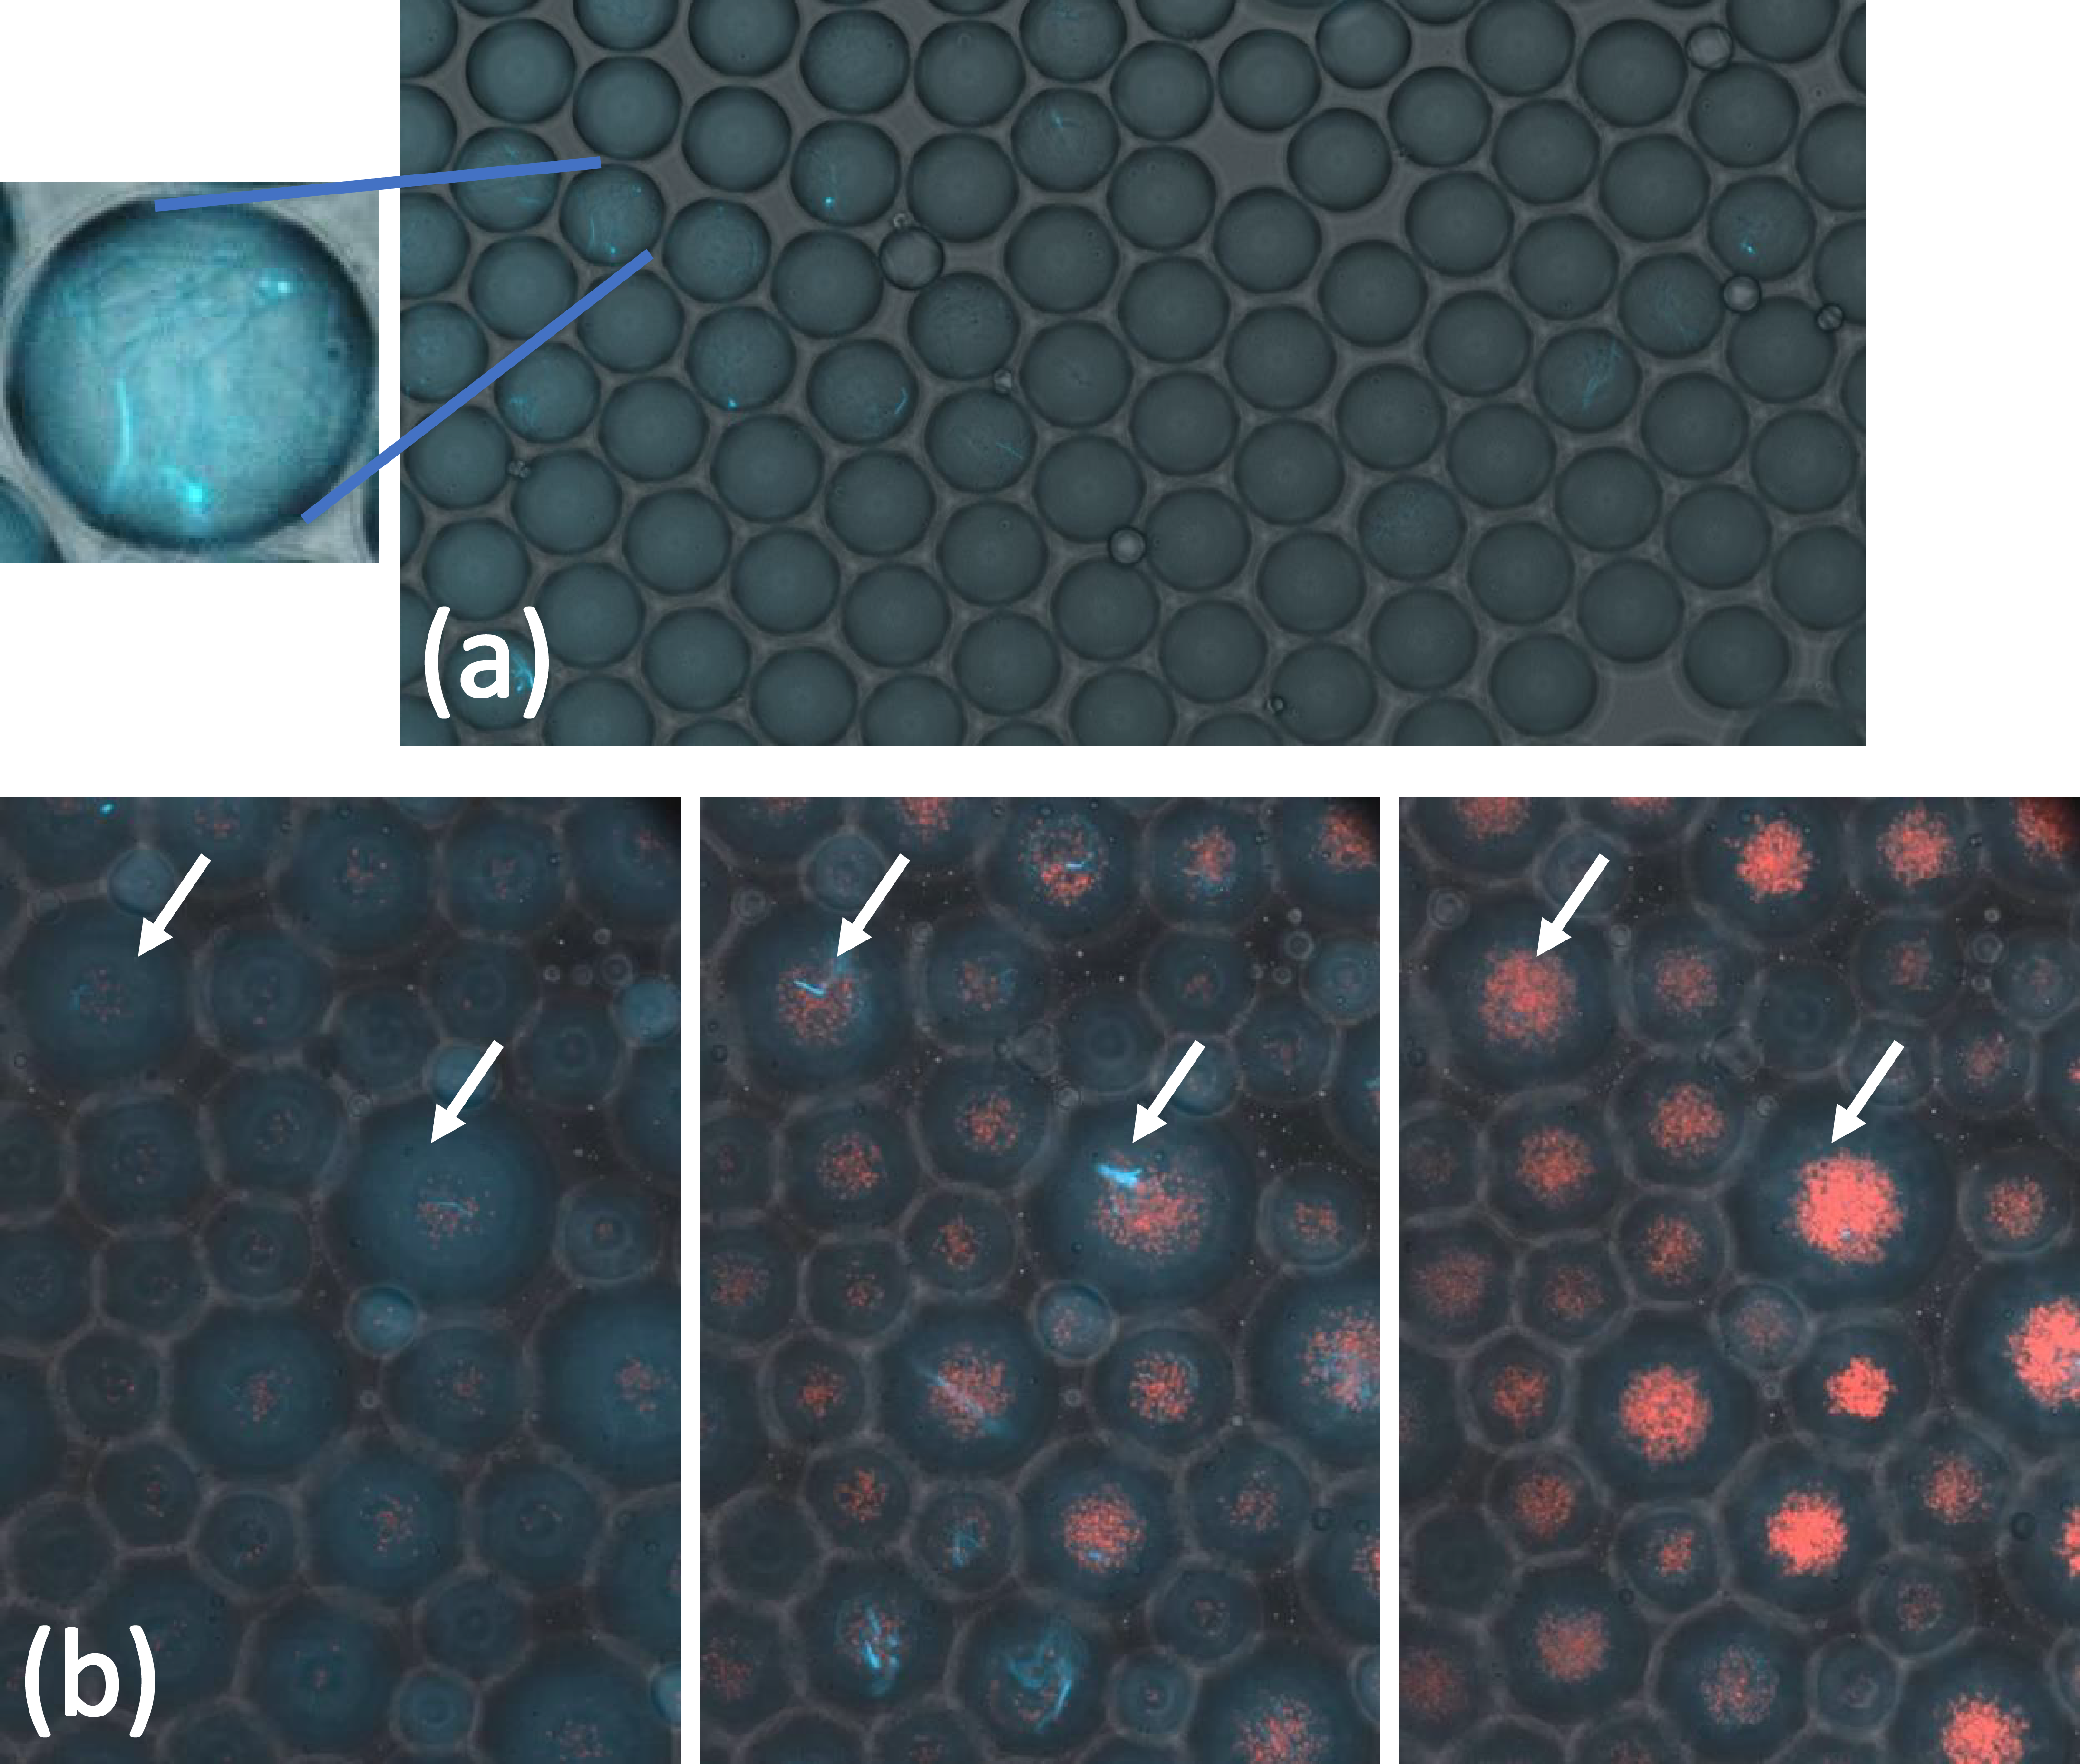
\includegraphics[width=\linewidth]{graphics/2025_09_30_droplets_fig8.png}
\caption{\textbf{On-chip droplets are stable after long-term incubation and allow bacterial growth} Our setup allows for long-term incubation and monitoring of droplets. (a) shows the results after 21h of incubation of droplets containing antibiotic producers alone in 30$^\circ$C. We observe stable same-sized droplets containing fluorescently tagged bacteria. The bacteria seem to be stressed and filament in the droplets as can be seen in the contrast and brightness enhanced enlarged droplet on the left. (b) shows snapshots of a time series of droplets containing both, antibiotic producing \textit{B. subtilis} (tagged in blue) and sensitive \textit{S. aureus} (tagged in red). Initially we see growth of both bacterial strains. However, \textit{B. subtilis} seems to be filamenting (examples indicated with arrows) and at the end of the incubation, most droplets are filled exclusively with the target \textit{S. aureus} strain.}
\label{fig:results_incubation_subtilis}
\end{figure}
After establishing the technical platform, we can incubate droplets for long periods of time and can monitor them under the microscope during these incubation periods~(Figure~\ref{fig:results_incubation_subtilis}). We encapsulate the antibiotic producer alone~(shown after incubation in Figure~\ref{fig:results_incubation_subtilis}a) and together with the target strain (time series in Figure~\ref{fig:results_incubation_subtilis}b) in droplets. Encapsulating it alone, we observe long filaments of cells in the droplets after incubation as the enlarged, contrast and brightness enhanced droplet in the figure shows. This indicates some kind of stress in this specific growth environment. When encapsulating it together with sensitive bacteria, we observe droplets with antibiotic producers and target cells and some only with target cells, in line with the chosen concentrations. After initial growth, we observe filamenting antibiotic producers (marked with white arrows in the time series in Figure~\ref{fig:results_incubation_subtilis}b) and after 21h of incubation, the antibiotic producers disappeared almost completely from the droplets (Figure~\ref{fig:results_incubation_subtilis}b, right side), while the target cells grow properly in the droplets. Together with the observation of filaments in droplets where antibiotic producers are encapsulated alone, this might indicate the lack of toxin production and the lack of growth of antibiotic producers in droplets.

\section{Comparison of growth in liquid and droplet environment}
To understand if the antibiotic producer disappears only in droplets or also in liquid, we performed a liquid-droplet comparison assay with separate cultures of antibiotic producer and the target strain. After incubation for 21h with high inoculation densities, we see that both liquid cultures exhibited growth while in droplets only the target strain exhibits growth. The antibiotic producer seems to not grow in droplets during the incubation period but rather seems to reduce in population size~(Figure~\ref{fig:results_liquid_vs_drop_supernatant}a).

\begin{figure}
\centering
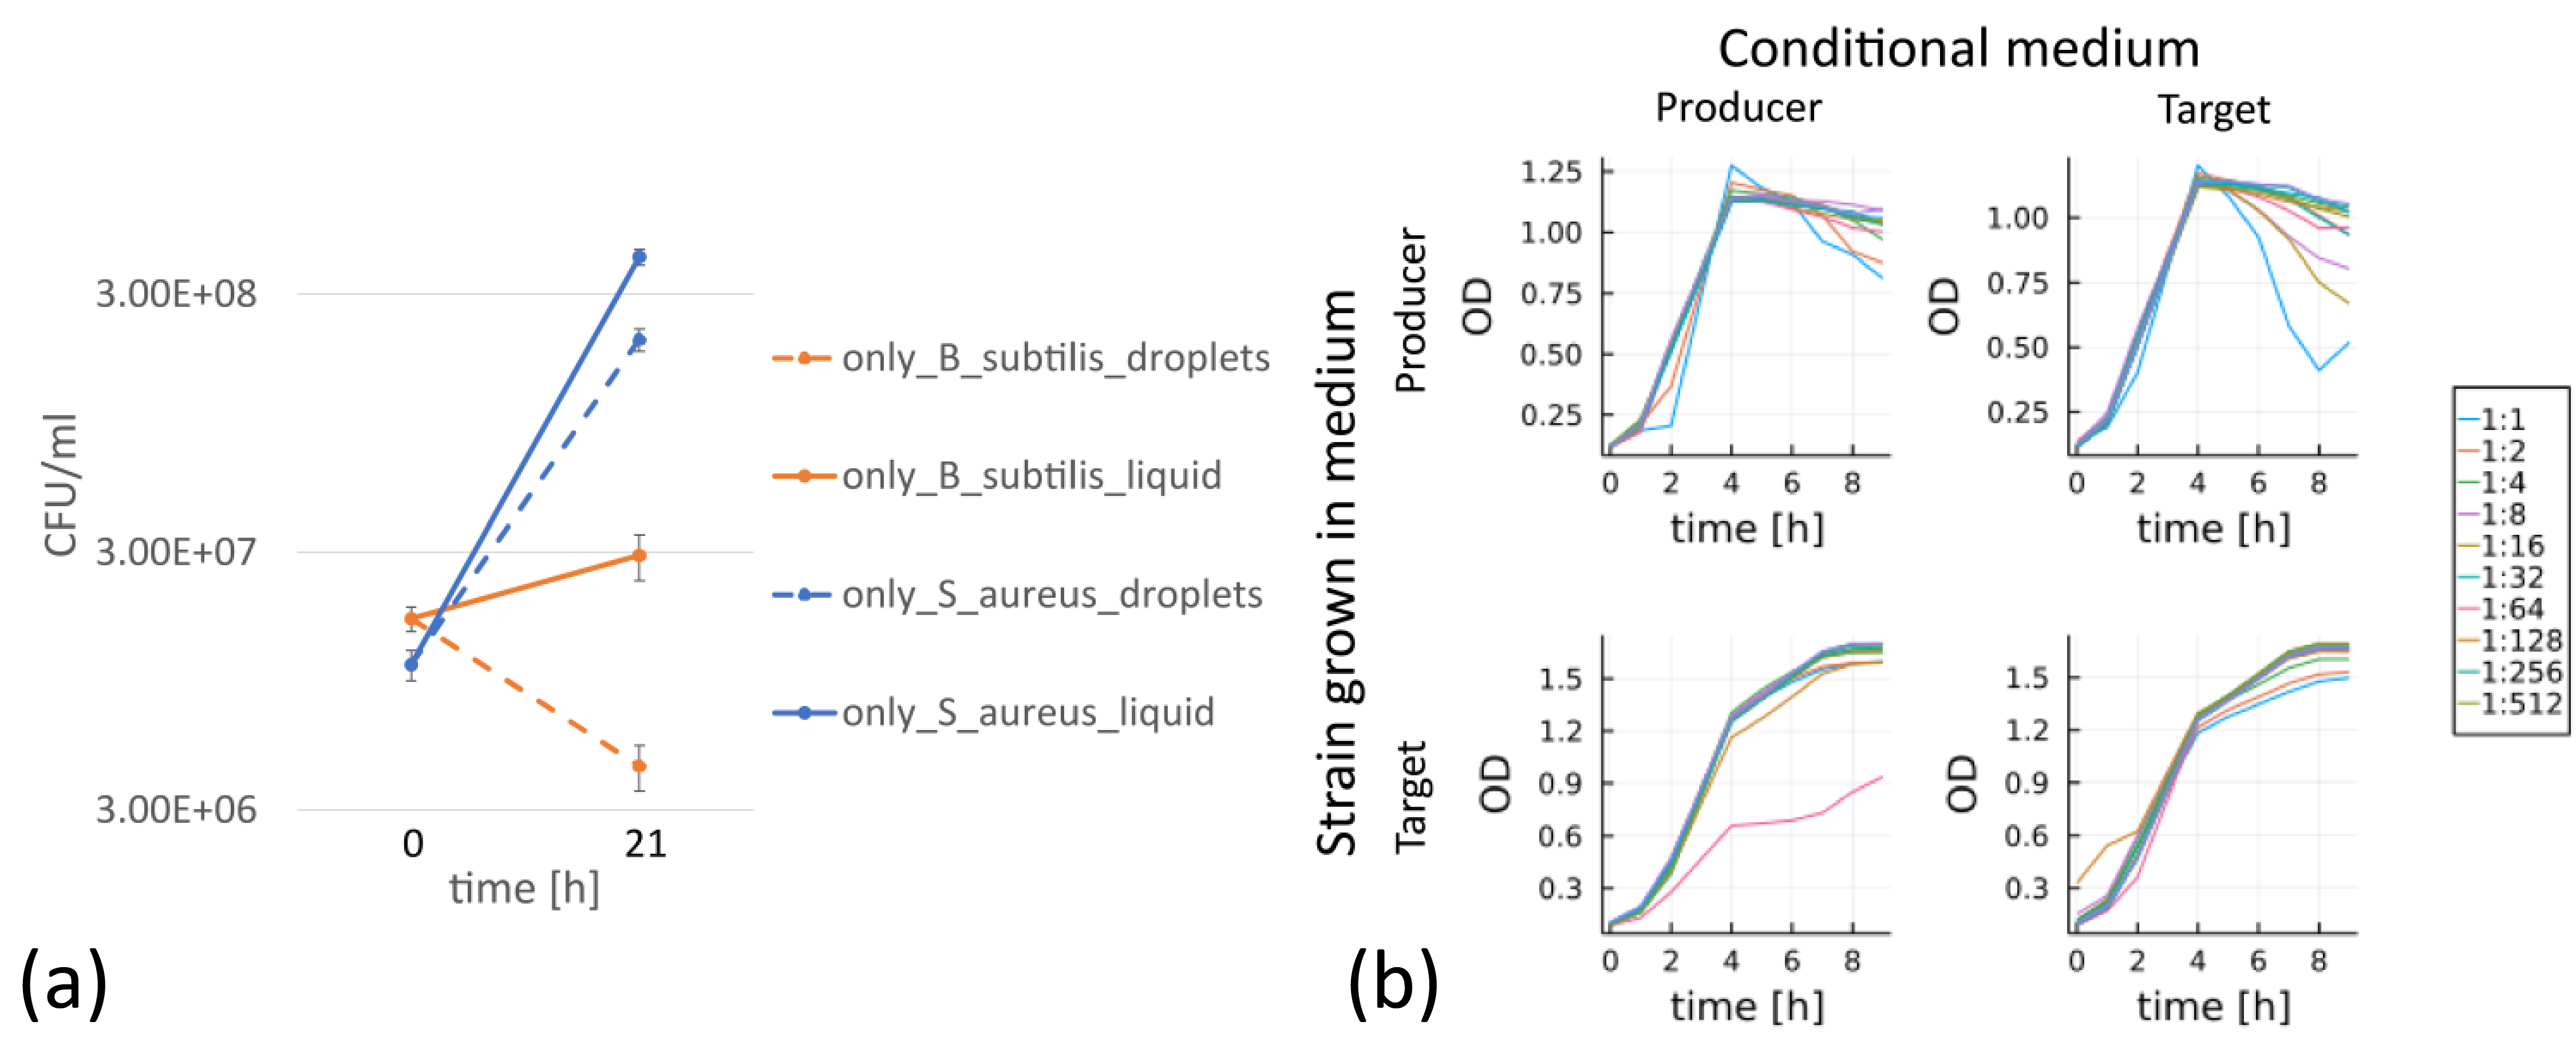
\includegraphics[width=\linewidth]{graphics/2025_09_30_droplets_fig9.png}
\caption{\textbf{\textit{B. subtilis} fails to grow in droplets and does not kill in liquid} To understand the observed dynamics in droplets, we conducted liquid experiments. (a) shows the results of comparing growth of antibiotic producing \textit{B. subtilis} alone (orange) in liquid (solid line) and in droplets (dashed line) and similarly for the target \textit{S. aureus} strain (blue). We observe that \textit{B. subtilis} seems to die in droplets while it grows in liquid culture. \textit{S. aureus} seems to grow almost equally well in droplets and liquid culture. (b) shows the results of growing bacteria in conditional medium. Studying both, antibiotic producer and target strain conditional media, we do not observe an effect of the antibiotic in liquid, hinting at the possible absence of antibiotic in liquid compared to growth on agar.}
\label{fig:results_liquid_vs_drop_supernatant}
\end{figure}

\section{Chosen antibiotic producer does not produce sufficient antibiotic to kill target strain in conditional medium}
To measure the effectivity of the produced antibiotic, we use a conditional medium assay. We grow producer and target on its own or the other strain's conditional medium respectively. We do not observe a significant impact of the conditional medium on growth of bacteria in any of the conditions~(Figure~\ref{fig:results_liquid_vs_drop_supernatant}b), especially when growing the target strain on the conditional medium of the antibiotic producing strain~(Figure~\ref{fig:results_liquid_vs_drop_supernatant}b, bottom left). This indicates the lack of significant antibiotic production by the producer when grown in liquid, rendering it unusable in a droplet encapsulation scenario.